\documentclass[oneside,numbers,spanish]{ezthesis}
\usepackage[utf8]{inputenc}
\usepackage{graphicx}
\usepackage{float}
\usepackage[rflt]{floatflt}
%% # Opciones disponibles para el documento #
%%
%% Las opciones con un (*) son las opciones predeterminadas.
%%
%% Modo de compilar:
%%   draft            - borrador con marcas de fecha y sin im'agenes
%%   draftmarks       - borrador con marcas de fecha y con im'agenes
%%   final (*)        - version final de la tesis
%%
%% Tama'no de papel:
%%   letterpaper (*)  - tama'no carta (Am'erica)
%%   a4paper          - tama'no A4    (Europa)
%%
%% Formato de impresi'on:
%%   oneside          - hojas impresas por un solo lado
%%   twoside (*)      - hijas impresas por ambos lados
%%
%% Tama'no de letra:
%%   10pt, 11pt, o 12pt (*)
%%
%% Espaciado entre renglones:
%%   singlespace      - espacio sencillo
%%   onehalfspace (*) - espacio de 1.5
%%   doublespace      - a doble espacio
%%
%% Formato de las referencias bibliogr'aficas:
%%   numbers          - numeradas, p.e. [1]
%%   authoryear (*)   - por autor y a'no, p.e. (Newton, 1997)
%%
%% Opciones adicionales:
%%   spanish         - tesis escrita en espa'nol
%%
%% Desactivar opciones especiales:
%%   nobibtoc   - no incluir la bibiolgraf'ia en el 'Indice general
%%   nofancyhdr - no incluir "fancyhdr" para producir los encabezados
%%   nocolors   - no incluir "xcolor" para producir ligas con colores
%%   nographicx - no incluir "graphicx" para insertar gr'aficos
%%   nonatbib   - no incluir "natbib" para administrar la bibliograf'ia

%% Paquetes adicionales requeridos se pueden agregar tambi'en aqu'i.
%% Por ejemplo:
%\usepackage{subfig}
%\usepackage{multirow}

%% # Datos del documento #
%% Nota que los acentos se deben escribir: \'a, \'e, \'i, etc.
%% La letra n con tilde es: \~n.

\author{\textbf{Luis Ignacio García Reyes}}
\title{\large{Diseño e implementación de un electrocardiograma con aplicación en sistema Android.}}
\degree{\textit{Calidad en las telecomunicaciones}}
%\supervisor{Nombre de mi Asesor}
\institution{\huge{Universidad Autónoma De La Ciudad de México}}
\faculty{}
\department{Ingeniería en sistemas electrónicos y de telecomunicaciones}

%% # M'argenes del documento #
%% 
%% Quitar el comentario en la siguiente linea para austar los m'argenes del
%% documento. Leer la documentaci'on de "geometry" para m'as informaci'on.

%\geometry{top=40mm,bottom=33mm,inner=40mm,outer=25mm}

%% El siguiente comando agrega ligas activas en el documento para las
%% referencias cruzadas y citas bibliogr'aficas. Tiene que ser *la 'ultima*
%% instrucci'on antes de \begin{document}.
\hyperlinking
\begin{document}

%% En esta secci'on se describe la estructura del documento de la tesis.
%% Consulta los reglamentos de tu universidad para determinar el orden
%% y la cantidad de secciones que debes de incluir.

%% # Portada de la tesis #
%% Mirar el archivo "titlepage.tex" para los detalles.

%% ## Construye tu propia portada ##
%% 
%% Una portada se conforma por una secuencia de "Blocks" que incluyen
%% piezas individuales de informaci'on. Un "Block" puede incluir, por
%% ejemplo, el t'itulo del documento, una im'agen (logotipo de la universidad),
%% el nombre del autor, nombre del supervisor, u cualquier otra pieza de
%% informaci'on.
%%
%% Cada "Block" aparece centrado horizontalmente en la p'agina y,
%% verticalmente, todos los "Blocks" se distruyen de manera uniforme 
%% a lo largo de p'agina.
%%
%% Nota tambi'en que, dentro de un mismo "Block" se pueden cortar
%% lineas usando el comando \\
%%
%% El tama'no del texto dentro de un "Block" se puede modificar usando uno de
%% los comandos:
%%   \small      \LARGE
%%   \large      \huge
%%   \Large      \Huge
%%
%% Y el tipo de letra se puede modificar usando:
%%   \bfseries - negritas
%%   \itshape  - it'alicas
%%   \scshape  - small caps
%%   \slshape  - slanted
%%   \sffamily - sans serif
%%
%% Para producir plantillas generales, la informaci'on que ha sido inclu'ida
%% en el archivo principal "tesis.tex" se puede accesar aqu'i usando:
%%   \insertauthor
%%   \inserttitle
%%   \insertsupervisor
%%   \insertinstitution
%%   \insertdegree
%%   \insertfaculty
%%   \insertdepartment
%%   \insertsubmitdate

\begin{titlepage}
  \TitleBlock{\scshape\insertinstitution}
  \TitleBlock[\bigskip]{\scshape\insertfaculty}
  \TitleBlock{\Huge\scshape\inserttitle}
  \TitleBlock{\scshape
    Trabajo presentado por \insertauthor \\
    para certificar la materia  de \insertdegree}
  \TitleBlock{\insertsubmitdate}
  \TitleBlock[\bigskip]{\insertdepartment}
\end{titlepage}

%% Nota 1:
%% Se puede agregar un escudo o logotipo en un "Block" como:
%%   \TitleBlock{\includegraphics[height=4cm]{escudo_uni}}
%% y teniendo un archivo "escudo_uni.pdf", "escudo_uni.png" o "escudo_uni.jpg"
%% en alg'un lugar donde LaTeX lo pueda encontrar.

%% Nota 2:
%% Normalmente, el espacio entre "Blocks" se extiende de modo que el
%% contenido se reparte uniformemente sobre toda la p'agina. Este
%% comportamiento se puede modificar para mantener fijo, por ejemplo, el
%% espacio entre un par de "Blocks". Escribiendo:
%%   \TitleBlock{Bloque 1}
%%   \TitleBlock[\bigskip]{Bloque2}
%% se deja un espacio "grande" y de tama~no fijo entre el bloque 1 y 2.
%% Adem'as de \bigskip est'an tambi'en \smallskip y \medskip. Si necesitas
%% aun m'as control puedes usar tambi'en, por ejemplo, \vspace*{2cm}.




%% # Prefacios #
%% Por cada prefacio (p.e. agradecimientos, resumen, etc.) crear
%% un nuevo archivo e incluirlo aqu'i.
%% Para m'as detalles y un ejemplo mirar el archivo "gracias.tex".
%%% Las secciones del "prefacio" inician con el comando \prefacesection{T'itulo}
%% Este tipo de secciones *no* van numeradas, pero s'i aparecen en el 'indice.
%%
%% Si quieres agregar una secci'on que no vaya n'umerada y que *tampoco*
%% aparesca en el 'indice, usa entonces el comando \chapter*{T'itulo}
%%
%% Recuerda que aqu'i ya puedes escribir acentos como: 'a, 'e, 'i, etc.
%% La letra n con tilde es: 'n.

\prefacesection{Agradecimientos}

Este apartado únicamente lo he dejado en blanco para simular el contenido que mas adelante agregare.

%% Por si alguien tiene curiosidad, este "simp'atico" agradecimiento est'a
%% tomado de la "Tesis de Lydia Chalmers" basada en el universo del programa
%% de televisi'on Buffy, la Cazadora de Vampiros.
%% http://www.buffy-cazavampiros.com/Spiketesis/tesis.inicio.htm


%% # 'Indices y listas de contenido #
%% Quitar los comentarios en las lineas siguientes para obtener listas de
%% figuras y cuadros/tablas.


\tableofcontents

\listoffigures
 % para que aparezca en el indice de contenidos
 % indice de figuras
%\listoffigures
%\listoftables

\prefacesection{Justificación}
La tecnología actualmente evoluciona continuamente y de forma acelerada mostrando mas dispositivos de  mayores funciones y con mayores recursos, por ende, pensar en la construcción de un circuito que promueva el uso de la medicina general en un rubro especifico para la sociedad en general no es una idea que no pase por alto, en este caso hablando en particular del EGC en cuestión, nos permite mostrar la idea que deseamos expresar, la situación actual de México es de una población de jóvenes en su mayoría, sin embargo estas cifras (Véase cifras del INEGI) se modificaran con el tiempo y en unas décadas se pasara de un país de jóvenes a un país de adultos, sin embargo, esto nos da una idea de hacia donde se dirige la situación del país y que elementos debemos tomar en cuenta para la creación de nuevos circuitos que ayuden a la población, pensando en esto la creación de un EGC que nos permita conectarse con un teléfono celular y realizar un monitoreo  del corazón, es una idea que busca el acceso de nuevas herramientas en materia de medicina para que el usuario pueda observar de manera practica su evolución sin consultar directamente una clínica que no necesariamente este dentro de su localidad.\newline\par

Por otra parte la evolución tecnológica ha sufrido cambios sustanciales con respecto a cada generación de dispositivos, esto, ha aumentado las capacidades técnicas de cada dispositivo y por ende las funciones que estos pueden realizar, a pesar de los esfuerzos que se han impuestos en estos dispositivos, el presentar nuevas herramientas para distintas funciones ha sido un reto de hoy en día para los teléfonos celulares de ultima generación debido a que los desarrolladores no están familiarizados con todas las áreas de investigación y esto abre las puertas a que ingenieros de todas las ramas puedan aportar sus conocimientos para aplicarlos de manera mas practica.
%%% Los cap'itulos inician con \chapter{T'itulo}, estos aparecen numerados y
%% se incluyen en el 'indice general.
%%
%% Recuerda que aqu'i ya puedes escribir acentos como: 'a, 'e, 'i, etc.
%% La letra n con tilde es: 'n.

\prefacesection{Objetivos}
\textbf{Objetivo general}
Construir un electrocardiograma que nos permita reducir en tamaño un electrocardiograma convencional y realizar una interfaz para conectarse con un teléfono celular con sistema operativo Android.\newline\par
\textit{Objetivos particulares}
\begin{itemize}
\item Comprender el funcionamiento de un EGC en su diagrama a bloques.
\item Elegir los componentes correcto para la construcción del EGC.
\item Comparar los resultados con un EGC.
\item Maquetación de aplicación en Android.
\item Realización de la aplicación en API 21.
\item Presentación final.
\end{itemize}

%% # Cap'itulos #
%% Por cada cap'itulo hay que crear un nuevo archivo e incluirlo aqu'i.
%% Mirar el archivo "intro.tex" para un ejemplo y recomendaciones para
%% escribir.
%
\prefacesection{Justificación}
La tecnología actualmente evoluciona continuamente y de forma acelerada mostrando mas dispositivos de  mayores funciones y con mayores recursos, por ende, pensar en la construcción de un circuito que promueva el uso de la medicina general en un rubro especifico para la sociedad en general no es una idea que no pase por alto, en este caso hablando en particular del EGC en cuestión, nos permite mostrar la idea que deseamos expresar, la situación actual de México es de una población de jóvenes en su mayoría, sin embargo estas cifras (Véase cifras del INEGI) se modificaran con el tiempo y en unas décadas se pasara de un país de jóvenes a un país de adultos, sin embargo, esto nos da una idea de hacia donde se dirige la situación del país y que elementos debemos tomar en cuenta para la creación de nuevos circuitos que ayuden a la población, pensando en esto la creación de un EGC que nos permita conectarse con un teléfono celular y realizar un monitoreo  del corazón, es una idea que busca el acceso de nuevas herramientas en materia de medicina para que el usuario pueda observar de manera practica su evolución sin consultar directamente una clínica que no necesariamente este dentro de su localidad.\newline\par

Por otra parte la evolución tecnológica ha sufrido cambios sustanciales con respecto a cada generación de dispositivos, esto, ha aumentado las capacidades técnicas de cada dispositivo y por ende las funciones que estos pueden realizar, a pesar de los esfuerzos que se han impuestos en estos dispositivos, el presentar nuevas herramientas para distintas funciones ha sido un reto de hoy en día para los teléfonos celulares de ultima generación debido a que los desarrolladores no están familiarizados con todas las áreas de investigación y esto abre las puertas a que ingenieros de todas las ramas puedan aportar sus conocimientos para aplicarlos de manera mas practica.
%% Los cap'itulos inician con \chapter{T'itulo}, estos aparecen numerados y
%% se incluyen en el 'indice general.
%%
%% Recuerda que aqu'i ya puedes escribir acentos como: 'a, 'e, 'i, etc.
%% La letra n con tilde es: 'n.

\prefacesection{Objetivos}
\textbf{Objetivo general}
Construir un electrocardiograma que nos permita reducir en tamaño un electrocardiograma convencional y realizar una interfaz para conectarse con un teléfono celular con sistema operativo Android.\newline\par
\textit{Objetivos particulares}
\begin{itemize}
\item Comprender el funcionamiento de un EGC en su diagrama a bloques.
\item Elegir los componentes correcto para la construcción del EGC.
\item Comparar los resultados con un EGC.
\item Maquetación de aplicación en Android.
\item Realización de la aplicación en API 21.
\item Presentación final.
\end{itemize}

%%Aqui agregare lo que sera el marco teorico
%%Ademas de algunas modificaciones que se vallan presentando
%% Los cap'itulos inician con \chapter{T'itulo}, estos aparecen numerados y
%% se incluyen en el 'indice general.
%%
%% Recuerda que aqu'i ya puedes escribir acentos como: 'a, 'e, 'i, etc.
%% La letra n con tilde es: 'n.

\chapter{Introducción}
Las actividades a realizar en este proyecto son una serie de consecuencias dentro de las nuevas tecnologías que se implementan a diario como nuevos proyectos, los resultados de estos proyectos (antecedentes a este) han sido bases para nuevas tecnologías e innovación, a pesar de esto nuevas y mas preguntas resultan de los nuevos elementos por ejemplo con el EGC se realiza una cuestión de utilidad y que beneficios contrae a las partes que utilizarían este dispositivo, sin embargo un énfasis que aborda el análisis de la utilidad de los dispositivos dispone que entre mas nos enfoquemos en la tecnología mas dudas surgen y por ello el proponer una nueva utilidad es un rubro muy importante, se propone que un dispositivo celular sea útil para poder dar mas herramientas a la vida cotidiana actual, lo cual, es sinónimo de avances tecnológicos ya que demanda mas recursos por parte de los dispositivos para poder ofertar mas servicios, en particular la telefonía celular es el claro ejemplo de este avance.

En la medicina actual en México es evidente que hace falta mucha investigación y recursos para poder dar cauce a investigaciones mas profundas en materia de cardiología, a pesar de que no es un rubro que cauce muertes en enormes cantidades debemos hacer énfasis en que existen pocas herramientas para el chequeo cotidiano y que las existentes requieren que la persona se traslade desde su localidad a un hospital cercano que cuente con los dispositivos de medición.




\chapter{Antecedentes}
\textit{El presente trabajo presenta la construcción de un electrocardiograma convencional utilizando conocimientos de programación en PIC's y adaptando una interfaz en un teléfono con sistema operativo android.}\newline
\textit{Los elementos que vamos a utilizar son:}
\begin{itemize}
\item \textit{Baterias 12V}
\item \textit{Regulador de tension LM317T}
\item \textit{TTL 74LS04}
\item \textit{PIC18F4550}
\item \textit{Electrodos}
\item \textit{Cables para electrocardiografía}
\item \textit{Adaptadores para cables electrocardiógrafos}
\end{itemize}
Así como se puede consultar en el trabajo recepcional de tesis de Guillermo Eduardo Vega Picón

\begin{figure}
   	\centering
		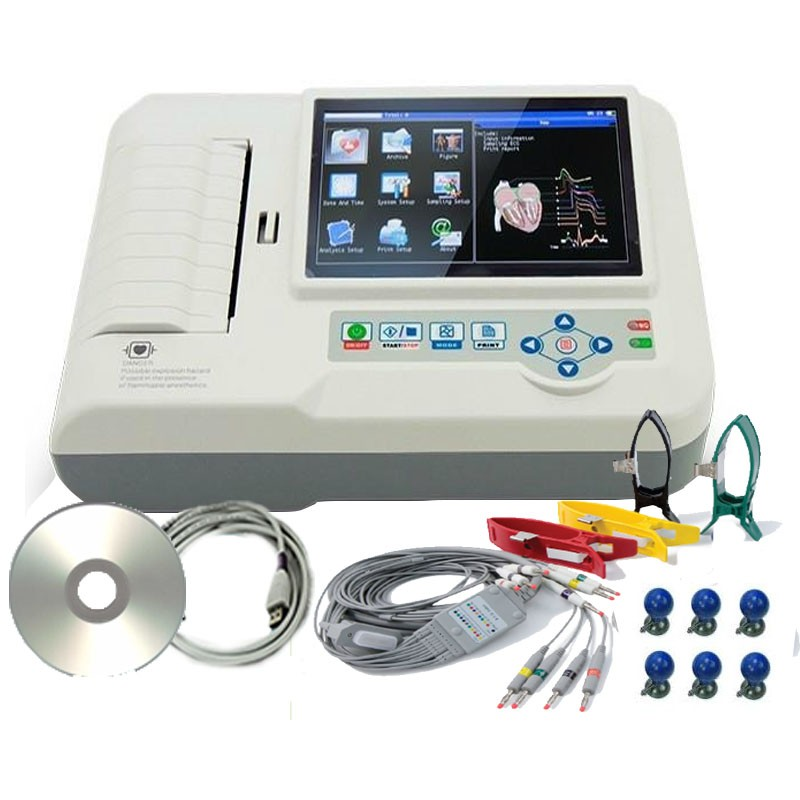
\includegraphics[width=12cm]{imag/electrocardiografo.jpg}
		\caption{Electrocardiografo.}
		\label{cavi}
\end{figure}
%\include{capitulo1}
%\include{capitulo2}
%\include{capitulo3}
%\include{conclu}
%% Los cap'itulos inician con \chapter{T'itulo}, estos aparecen numerados y
%% se incluyen en el 'indice general.
%%
%% Recuerda que aqu'i ya puedes escribir acentos como: 'a, 'e, 'i, etc.
%% La letra n con tilde es: 'n.
\chapter{Corazón y sus características}

El corazón es uno de los órganos mas importantes del cuerpo humano ya que es el encargado de bombear sangre a través de las venas por todo el cuerpo, tiene como dimensiones, 12 centímetros de largo, 9 centímetros de ancho y 6 centímetros de espesor, su peso ronda entre los 200 y 425 gramos.\newline

\begin{floatingfigure}[r]{3cm}

\includegraphics{imag/corazon.PNG}
%\captionof{Figura}{Un poliedro}
\end{floatingfigure}

Como tal esta formado por dos bombas que se les menciona como corazón derecho e izquierda el primero bombea sangre hacia los pulmones y el izquierdo bombea sangre por la circulación sistémica que lo lleva hacia los demás órganos del cuerpo.\newline
Se encuentra ubicado en la región del mediastino medio, justo entre los pulmones y la parte media del pecho, detrás del esternón, se apoya sobre el diafragma.\newline\newline
Como tal el corazón esta dividido en dos mitades incomunicadas entre si(Figura\ref{cavi}), una derecha y una izquierda, estas mitades se subdividen en dos cavidades conformando un total de 4 cavidades, la capa superior se llama aurícula y la cavidad inferior se llama ventrículo.\newline

En la figura \ref{cavi} observamos los principales componentes de las cavidades del corazón, estas son las partes mas importantes para obtener las señales correspondientes, esto ya que el corazón no tiene un movimiento  uniforme, si no que cada componente forma un patrón consecutivo en el cual su señal es independiente pero es consecuencia de un antecesor.

\begin{figure}[H]
   	\centering
		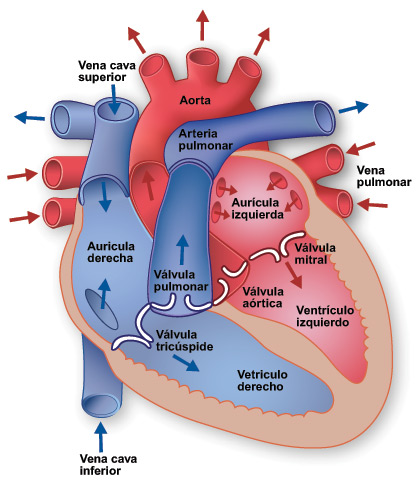
\includegraphics[width=6cm]{imag/cavidad.jpg}
		\caption{Cavidades.}
		\label{cavi}
\end{figure}


Como tal para que el corazón se contraiga es necesario que sus células musculares reciban un estímulo eléctrico. Este se genera en células especializadas (células marca pasos) del sistema de conducción, que originan el impulso por sufrir des polarizaciones espontáneas (automatismo).\newline

Cada cara del corazón la exploran unas derivaciones particulares: inferior(II, III, aVF), lateral alta (I, aVL), lateral baja (V5,v6), anterior(V3, V4), septo (V1, V2), posterior(V7,V8,V9), ventrículo derecho (V3R, V4R).
\chapter{Componentes electrónicos}
Dentro de los componentes mas importantes se encuentran los siguientes:\newline

\textit{Electrodos}: estos elementos son los encargados de recibir la señal proveniente del cuerpo humano (Figura 4.1), se adhiere a la piel y se agrega un desinfectante para evitar ruido para la señal.\newline
\begin{floatingfigure}[r]{4.5cm}
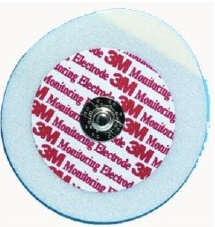
\includegraphics{imag/electrodo.PNG}
%\captionof{Figura}{Un poliedro}
\caption{Electrodos.}
		\label{electrodos}
\end{floatingfigure}

\textit{Cables para electrocardiógrafo}, estos son los medios de transmisión a través de los cuales es envía la información (señales eléctricas del corazón) y que tienen un aislante para no recibir perturbaciones externas.\newline

Esto permite que la señal entrante no tenga dentro de si demasiado ruido y se permita un correcto análisis de esta. El acondicionamiento de la señal se debe en mucho a la correcta colocación de este elemento.\newline

\begin{floatingfigure}[r]{1.0cm}
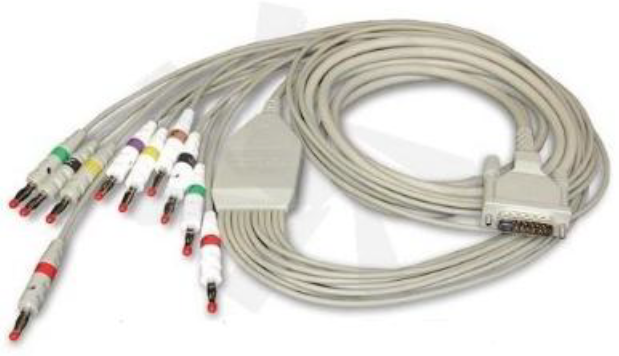
\includegraphics{imag/cables.PNG}
%\captionof{figure}{Un poliedro}
\end{floatingfigure}

\textit{Adaptadores}: Estos por su parte permiten que la señal que viene a través del medio de transmisión se incorpore al sistema para que el sistema interno ya trabaje con esta señal.\newpage
\begin{figure}[H]
   	\centering
		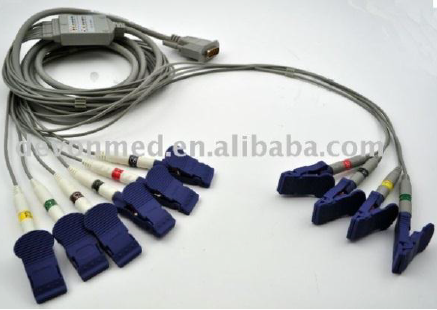
\includegraphics[width=6cm]{imag/adaptadores.PNG}
		\caption{Adaptadores.}
		\label{Adaptador}
\end{figure}
Por último tenemos el \textit{Smartphone}, este dispositivo puede ser de,cualquier modelo,gama y/o versión de Android. Esto debido a que se puede dar soporte a múltiples versiones de Android para que no tenga ningún problema de compatibilidad.\newline

Actualmente estos dispositivos ya poseen ciertas características de hardware como un procesador y memoria ram de buenas capacidades, por ello es que se adquiere la posibilidad de mostrar señales de electrocardiógrafo sin mayor problema, ya que otras aplicaciones para Android son mas demandantes y operan sin mayor problema.
\begin{figure}[H]
   	\centering
		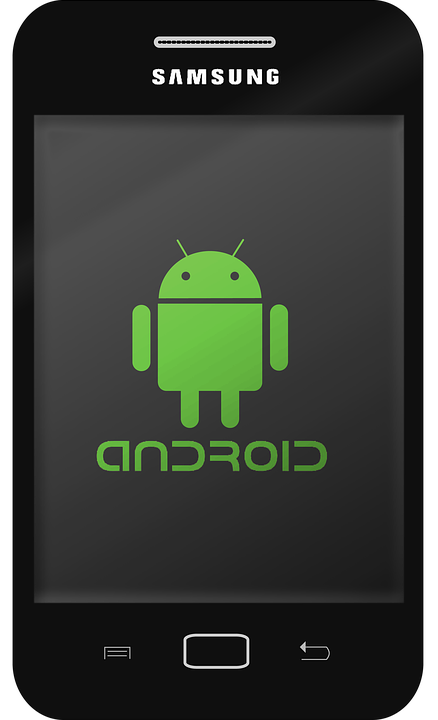
\includegraphics[width=3cm]{imag/smartphone.PNG}
		\caption{Smartphone.}
		\label{phone}
\end{figure}
\chapter{Sistema operativo Android}

El sistema operativo Android ó Android abreviandolo es un sistema de código abierto cuyo fin es desarrollar aplicaciones para teléfonos celulares y tabletas para el alcance de cualquier persona, es al igual que Linux, Ubuntu y otros sistemas un entorno que permite el desarrollo de nuevas herramientas sin fines de lucro, permite a los desarrolladores trabajar con entornos diseñados para la promoción del conocimiento.
\begin{floatingfigure}[r]{1cm}

\includegraphics{imag/mini.jpg}
%\captionof{figure}{Un poliedro}
\end{floatingfigure}
Para desarrollar una aplicación para Android se tienen distintas herramientas como lo son IDE´S (Entorno de Desarrollo Integrado) que facilitan la tarea de enlaces entre distintos lenguajes como lo son XML y java con las distintas clases que contiene dentro de si, esto da mayor empuje a las operaciones que se realizan dentro de las aplicaciones, sumado a esto tenemos que elegir una API (Interfaz de programación de aplicaciones).\newline

Una API dicho de manera cotidiana es la versión de Android que se posee en un dispositivo, está contiene distintas herramientas (o métodos) que se mejoran de una version a otra, corresponden a cada actualización del sistema y se les asigna un número.\newline
\begin{figure}
   	\centering
		
\includegraphics[width=4cm]{imag/androidmini.PNG}
		\caption{Android.}
		\label{andro}
\end{figure}
\newpage

Vamos a utilizar la API 21 para poder abarcar la mayor parte de dispositivos dentro de toda la gama de posibilidades. En particular para este proyecto utilizaremos Android Studio para desarrollar nuestra interfaz de usuario para visualizar las gráficas que se originen de nuestro circuito anterior.

%\include{capitulo1}
%\include{capitulo2}
%\include{capitulo3}
%\include{conclu}
\chapter{Implementación}
Como parte del desarrollo formal del proyecto se dan a elegir distintas opciones entre dispositivos para la captación de la señal proveniente del cuerpo humano, esto es claramente notable que se elige de una gama que va desde Raspberry Pi, Arduino, Pic´s (Familia 18F), módulos de E/S basados en sensor (de National Instruments), etc.\newline

Por ello debemos poner énfasis en el dispositivo correcto, en este caso se utilizará Pic de la familia 18F, debido a que tienen un buen procesamiento de datos, entrada analógica y convertidor A/D, junto con un lenguaje de programación manejable para el tipo de función que vamos a desempeñar.\newline
\begin{floatingfigure}[r]{3cm}
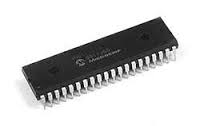
\includegraphics{imag/pic.jpg}
%\captionof{Figura}{Un poliedro}
\end{floatingfigure}


Aunque podemos utilizar los dispositivos antes mencionados, el tratamiento es el mismo únicamente se modifica la forma de atacar dichos datos y la salida respectiva, aunque no se descarta las funcionalidades que se tienen, en cierto modo se busca que este dispositivo sea practico y que pueda ser fácilmente utilizado, en este caso una persona que no dispone de los conocimientos previos para el manejo de Arduino o Raspberry evidentemente no aprovechara los recursos a comparación de un dispositivo que únicamente tenga como fin el de ser un EGC.\newpage

En términos simples toda señal (para proyectos de este tipo) recibida debe pasar por un tratamiento para poder apreciarla correctamente por el usuario final, se proponen una etapa de filtros y de acondicionamiento para que el proceso sea correcto, entre los que destacan se encuentran los que se muestran en las Figuras \ref{filtros} y \ref{filtros2}.

\begin{figure}[H]
\centering
\subfigure[A]{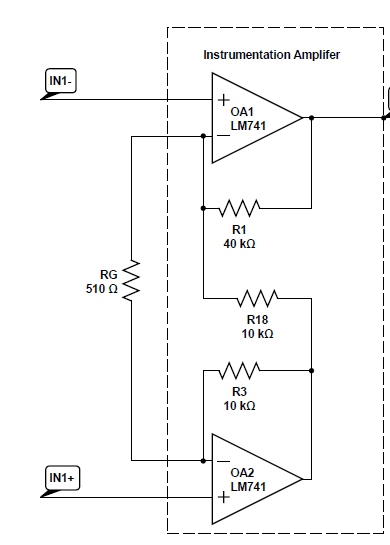
\includegraphics[scale=0.5]{imag/instrum.PNG}}
\subfigure[B]{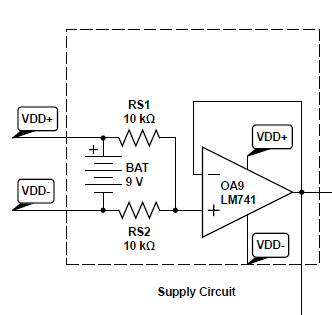
\includegraphics[scale=0.5]{imag/suply.PNG}}
\subfigure[C]{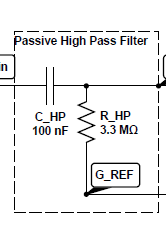
\includegraphics[scale=0.5]{imag/passive.PNG}}
\subfigure[D]{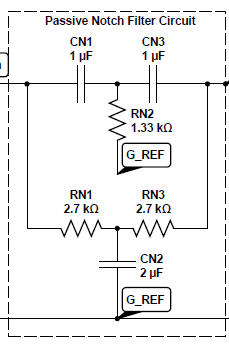
\includegraphics[scale=0.5]{imag/passive_notch.PNG}}
\caption{Filtros}
\label{filtros}
\end{figure}

\begin{figure}[H]
\centering
\subfigure[E]{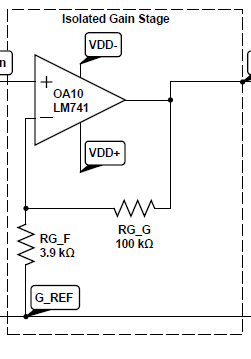
\includegraphics[scale=0.5]{imag/isolated_gain.PNG}}
\subfigure[F]{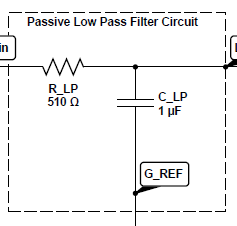
\includegraphics[scale=0.5]{imag/passive_low.PNG}}
\subfigure[G]{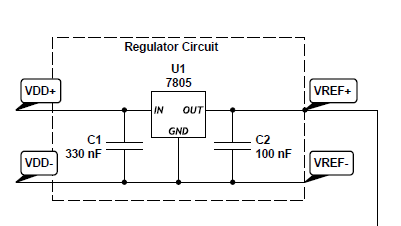
\includegraphics[scale=0.5]{imag/regulator.PNG}}
\subfigure[H]{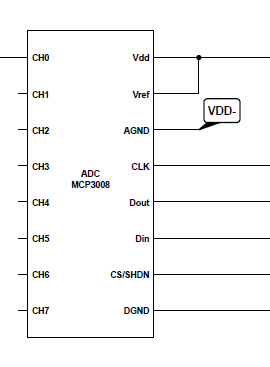
\includegraphics[scale=0.5]{imag/ADC.PNG}}
\caption{Filtros 2}
\label{filtros2}
\end{figure}
Donde cada parte se define como:
\begin{itemize}
\item[[A]] Amplificador de instrumentación.
\item[[B]] Circuito de suministro de poder.
\item[[C]] Filtro pasa-altas.
\item[[D]] Filtro pasivo notch.
\item[[E]] Etapa de ganancia.
\item[[F]] Filtro pasa-bajas.
\item[[G]] Circuito regulador.
\item[[H]] Convertidor A/D.
\end{itemize}
Estas etapas son en su mayoría recomendaciones de otros trabajos para poder realizar un proceso adecuado en la señal, aunque se consiguiera evitar alguna etapa se espera que se incluyan todas ya que esto seria optimo para un proceso integral y que no se pierda información o se le añada ruido.
\begin{figure}[H]
   	\centering
		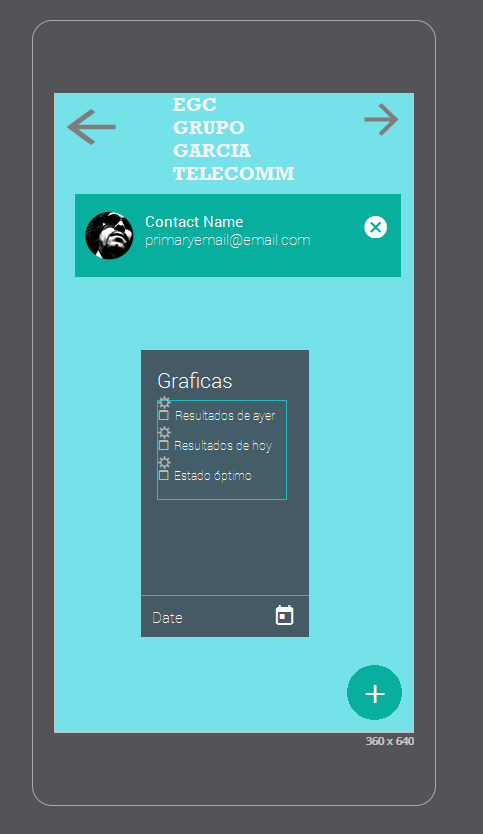
\includegraphics[width=6cm]{imag/app.PNG}
		\caption{Maquetación de la App en Android.}
		\label{app}
\end{figure}
La Figura \ref{app} es un ejemplo de como podría quedar la ventana de la aplicación esto se puede modificar fácilmente gracias a Android Studio y el software \textit{Justinmind} en este caso trabajamos con la \textit{Version (Ver. 7.5.0)}\newpage

Para la parte de interconexión entre elementos podemos utilizar un modulo embebido wifi como el que se muestra en la Figura \ref{wifi}, debemos tener en cuenta que el PIC de la familia 18F debe tener pines de TX y RX para poder enviar y recibir estas señales.
\begin{figure}[H]
   	\centering
		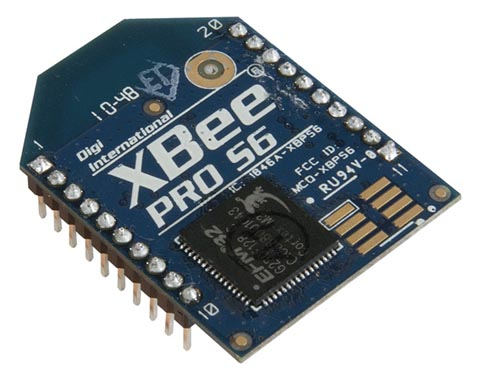
\includegraphics[width=6cm]{imag/wifi.jpg}
		\caption{Modulo embebido Wi-Fi.}
		\label{wifi}
\end{figure}

En este caso podemos utilizar el \textit{módulo embebido XBee de Digi International}, este que ofrece conectividad de serie a IEEE 802.11 (Wi-Fi).\newline

Este modulo responde a los requerimientos de bajo coste y mínimo consumo de redes inalámbricas con infraestructura 802.11, crea nuevas oportunidades en gestión de energía, automatización de procesos y factorías, sistemas de sensores, control inteligente de bienes y mercancías y otros muchos entornos, con lo cual es una buena elección de interconexión.




%\include{capitulo1}
%\include{capitulo2}
%\include{capitulo3}
\chapter{Conclusiones}
Como conclusión final tenemos que el avance en la tecnología se ha incrementado de forma ascendente en las últimas décadas, este dispositivo es un claro ejemplo de ello,por que nos demuestra que un EGC que hace apenas 10 años se actualiza en su forma de visualizar las señales de salida entonces tiene toda una ramificación de opciones a partir de las cuales se puede profundizar de muchas maneras, evidentemente el Internet de las cosas es un elemento que seguirá tomando auge en un futuro, por lo pronto para este proyecto se vislumbra como un paso mas.\newline

Dentro de las sugerencias mas notorias en impacto social que se pueden agregar a este proyecto serian:
\begin{itemize}
\item[*] El desarrollo de nuevos electrodos para evitar incomodidad.
\item[*] Permitir un multiplexaje del EGC para que permita atender a mas usuarios con un solo elemento.
\item[*] No solo trabajar con sistema operativo Android sino agregar mas sistemas.
\item[*] Llevar un registro de medico-paciente para llevar un mejor seguimiento del caso de un paciente
\end{itemize}
%\include{capitulo1}
%\include{capitulo2}
%\include{capitulo3}
\appendix
%% Cap'itulos incluidos despues del comando \appendix aparecen como ap'endices
%% de la tesis.
%\include{apendiceA}
%\include{apendiceB}
%\include{apendiceC}

%% Incluir la bibliograf'ia. Mirar el archivo "biblio.bib" para m'as detales
%% y un ejemplo.
\nocite{*}
\bibliographystyle{apalike}
\bibliography{ref}

\end{document}
